%Definir, caracterizar e mostrar um breve historico e as utilidades do foco



%Segue um exemplo de como INICIAR o texto. Da segunda palavra em
%diante, escreva normalmente
%	\IEEEPARstart{T}{his} demo file is intended to serve as a ``starter file''
%	for IEEE Computer Society journal papers produced under \LaTeX\ using
%	IEEEtran.cls version 1.7 and later.
%
%	\IEEEPARstart{D}{escrição}, com textos e imagens, da configuração do procedimento e cenário experimental. Explorar técnicas e métodos de medida 
%
\subsection{Objetivos}\label{obj}

\IEEEPARstart{E}{ste} experimento tem como objetivo a apresentação de um sinal de onda desconhecido. A apresentação poderá ser efetuada através de uma barra de LED's, displays de 7 segmentos ou com um LCD gráfico. É importante que a apresentação do sinal poderá ser feita de duas formas distintas. A primeira é o sinal exatamente da mesma forma como ele é colhido pelo MSP, a outra opção é utilizando um filtro, que pode ser representado pela equação \ref{filtro}.
	

\subsubsection{Material}\label{mat}
	
\begin{itemize}
	\item MSP430 LaunchPad
	\item Code Composer v4 ou MSPGCC
	\item MSP430G2553
	\item	\begin{itemize}
				\item 10x LED', ou
				\item 4 Displays de 7 segmentos, ou
				\item LCD Gráfico
			\end{itemize}
	\item Protoboard
\end{itemize}	
	
\subsection{Introdução Teórica}\label{intro}
%
%Exemplo de citação: \cite{msp430}
%

Para a realização deste experimento é importante a compreensão de um conversor AD (ADC). O que o conversor analógico/digital faz é capturar amostras do sinal analógico ao longo do tempo.
Cada amostra será convertida em um número, levando em consideração seu nível de tensão. 

\subsubsection{Taxa de Amostragem}\label{tax}

A frequência com que a amostragem irá ocorrer é chamada de taxa de amostragem. Se uma taxa de
amostragem de $22.050 Hz$ for usada, por exemplo, isto significa que em um segundo 22.050 pontos
serão capturados (ou sampleados ). A distância de cada ponto capturado será de $\frac{1}{22.050}$ segundo
(45,35$\mu$s, neste caso). Se a taxa de amostragem for de $44.100 Hz$, isto significa que 44.100 pontos
serão capturados por segundo. Neste caso a distância de cada ponto será de $\frac{1}{44.100}$ segundo ou
22,675$\mu$s, e assim por diante.\cite{cdh}

\subsubsection{Quantização}\label{quant}
Os valores instantâneos da tensão do sinal de entrada, que são obtidos na saída do circuito de amostragem e retenção precisam ser convertidos para a forma digital. Este processo recebe o nome de "quantização".
Os DSPs (Processadores Digitais de Sinais) processam os sinais analógicos convertidos para a forma digital e fazem uso deste processo.
O  que um DSP pode fazer com o sinal vai depender justamente da precisão com que a quantização é feita.
A representação dos valores instantâneos amostrados pelos circuitos anteriores depende do nível de quantização realizado, ou seja, quantos bits são usados para representar cada valor amostrado.
Assim, se usamos 2 bits teremos uma precisão menor do que se usarmos 4 bits para fazer a quantização.

\subsubsection{Resolução}\label{resolucao}

A resolução da conversão indica o número discreto de valores que podem ser produzidos sobre o intervalo de valores analógicos. Os valores são normalmente armazenados eletronicamente de forma binaria, assim a resolução é usualmente expressa em bits. Em consequência, o número de valores discretos disponíveis - níveis - são dados em potência de dois.

A resolução pode também ser definida eletricamente, e expressada em volts. A tensão mínima reconhecida pelo circuito é chamada de bit menos significativo - LSB (\textit{least significant bit}). A resolução (\textbf{Q}) do ADC é igual ao LSB. A voltagem de resolução é dada pela amplitude da tensão dividida pelo número de intervalos de voltagem discretas:

\[
	Q = \frac{E_{FSR}}{N}
\]
	
\begin{SCfigure}[1][h] %%Cuidado..ela não se mantem no lugar
  \centering
  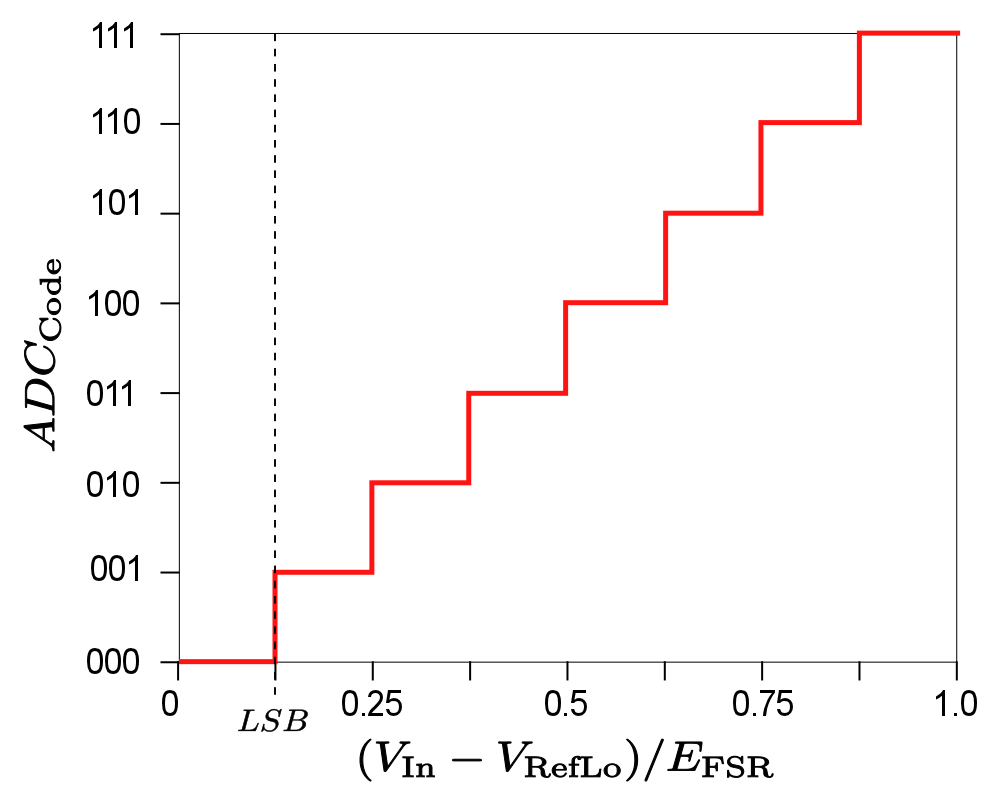
\includegraphics[width=5cm]{./fts/ADC}
  \caption{ Esquema de codificação ADC de 3 bits. Imagem de Wikipedia\cite{wikipedia}}
  \label{caption1}
\end{SCfigure}

Para o experimento, será aplicado um filtro que tem como função cortar as frequências mais altas, mostrando como saída um valor próximo da mediana. Ele pode ser representado pela equação \ref{filtro}, que é a média das quatro ultimas amostras:

\begin{equation}\label{filtro}
	Y=\frac{X_0+X_1+X_2+X_3}{4}
\end{equation}
